\chapter{Supremum, Infimum, and Completeness}\label{chapter:sup-inf-compl}
\vspace{12pt}

\section{Supremum and Infimum}

    \begin{theorem}\label{thm:supremum-property}
        Let $\emptyset \neq A \subseteq \bfR$. Let $u$ be an upperbound for $A$. The following are equivalent:
            \begin{enumerate}[label = (\arabic*)]
                \item $u = \Sup{(A)}$.
                \item If $t<u$, then there exists an $a_t \in A$ with $t < a_t$.
                \item For all $\epsilon > 0$, there exists an $a_\epsilon \in A$ such that $u - \epsilon < a_\epsilon$.
            \end{enumerate}
    \end{theorem}
        \begin{proof}
            $\left[(1)\implies(2)\right]$ Assume $u = \Sup{(A)}$. Let $t < u$. Suppose towards contradiction there does not exist and $a \in A$ with $a > t$. Then $a \leq t$ for all $a \in A$. But this implies $t$ is an upperbound of $A$ less than $u$, which is a contradiction because $u$ is the least upper bound. $\left[(2)\implies(3)\right]$ Given $\epsilon > 0$, let $t = u -\epsilon$. Then applying (2) gives the desired result. $\left[(3)\implies(1)\right]$ We know $u$ is an upperbound of $A$, we aim to show that it is the least upperbound. Let $v$ be an upperbound for $A$ with $ v < u$. Pick $\epsilon  = u - v > 0$. By (3), there exists an $a_\epsilon \in A$ such that $u - (u - v)  < a_\epsilon$. So $v < a_\epsilon$, which is a contradiction {\tiny( $v$ is an upperbound, how can it be smaller than an element of $A$?)}. 
        \end{proof}

    \begin{example}
        Claim: $\Sup([0,1)) = 1$. If $s \in [0,1)$, by definition $s<1$, so $1$ is an upper bound for $[0,1)$. Given $t<1$, set $\delta = 1-t > 0$. Then $0 < \frac{\delta}{2} < \delta$ {\color{red} this is not trivial, have to show $\delta - \delta/2$ is positive}. This gives:
            \begin{equation*}
            \begin{split}
                t < t+ \frac{\delta}{2} < t + \delta = 1.
            \end{split}
            \end{equation*}
        Pick $a_t = t + \frac{\delta}{2}$. By (2) of Theorem~\ref{thm:supremum-property}, $a_t \in [0,1)$, hence $1 = \Sup([0,1))$.
    \end{example}

    \begin{proposition}
        Let $A,B \subseteq \bfR$ and $a \leq b$ for all $a \in A$ and $b \in B$. Then $\Sup(A) \leq \Inf(B)$.
    \end{proposition}
        \begin{proof}
            Fix a point $b_0 \in B$. Then $a \leq b_0$ for all $a \in A$. Then $b_0$ is an upperbound for $A$. This gives $u := \Sup(A) \leq b_0$. But since $b_0$ was arbitrary, we have $u \leq b$ for all $b \in B$. So $u$ is a lower bound for $B$, therefore $u \leq \Inf(B)$.
        \end{proof}

    \begin{axiom}[Completeness of $\bfR$]
        Given any nonempty subset $A \subseteq \bfR$ which is bounded above, $\Sup(A)$ exists.
    \end{axiom}

    \begin{lemma}
        For $A \subseteq \bfR$ which is bounded below, $\sup(-A) = -\inf(A)$.
    \end{lemma}
        \begin{proof}
            If $A$ is bounded below, then $-A$ is bounded above. Then $\sup(-A)$ exists, define it as $u$. So for all $a \in A$, $-a \leq u$. Hence $-u$ is a lower bound for $A$. Suppose $v$ is another lower bound for $A$. Then $v \leq a$ for all $a \in A$. So $-v \geq -a$ for all $a \in A$. Thus $-v$ is an upper bound of $-A$. Therefore, since $u$ is the least upper bound, $-v \geq u$; i.e., $-u \geq v$. Thus $-u = \inf(A)$. 
        \end{proof}

    \begin{axiom}[Well-Ordering Princple]\label{axiom:wop}
        Every nonempty subset $A \subseteq \bfN$ contains a least element.
    \end{axiom}

    \begin{proposition}[Arcimedean Property 1]\label{prop:arch-1}
        If $x \in \bfR$, then there exists $n_x \in \bfN$ with $x < n_x$.
    \end{proposition}
        \begin{proof}
            Suppose not. That is, suppose $n \leq x$ for all $n \in \bfN$. Then $x$ is an upper bound for $\bfN$. Thus $\sup(A) := u$ exists. From part (3) of Theorem~\ref{thm:supremum-property}, take $\epsilon = 1$. Then there exists an $n \in \bfN$ such that $u - 1 < n$. So $u < n  + 1 \in \bfN$, which is a contradiction. 
        \end{proof}

    \begin{proposition}[Archimedean Property 2]\label{prop:arch-2}
        If $t > 0$, there exists $n_t \in \bfN$ with $\frac{1}{n_t} < t$.
    \end{proposition}
        \begin{proof}
            From \nameref{prop:arch-1}, pick $x = \frac{1}{t}$.
        \end{proof}

    \begin{corollary}
        Given $t>0$, there exists $m \in \bfN$ with $\frac{1}{2^m} < t$.
    \end{corollary}
        \begin{proof}
            By \nameref{prop:arch-2} there exists an $n \in \bfN$ with $\frac{1}{n} < t$. Claim: $\frac{1}{2^n} < \frac{1}{n}$. It suffices to show that $2^n > n$. Proposition~\ref{prop:power-set-bigger} gives $\card(\{1,2,...,n\}) < \card\left({\cP\left(\{1,2,...,n\}\right)}\right)$. Then Exercise~\ref{exercise:power-set-2n} gives:
                \begin{equation*}
                \begin{split}
                    n = \card(\{1,2,...,n\}) < \card\left({\cP\left(\{1,2,...,n\}\right)}\right) = 2^n.
                \end{split}
                \end{equation*}
            Alternatively, \nameref{prop:bernoulli} gives $(1+1)^n \geq 1 + n$. Hence $2^n > n$.
        \end{proof}

    \begin{example}
        \phantom{a}
        \begin{enumerate}[label = (\arabic*)]
            \item Claim: $\Inf{\left\{\frac{1}{n} \mid n \in N\right\}} = 0$. Note that $0$ is indeed a lower bound because $0 < \frac{1}{n}$ for all $n \in \bfN$. Suppose $t$ is another lower bound. If $t \leq 0$, then we are done. If $t > 0$, by the Archimedean Property there exists an $n_t \in \bfN$ such that $\frac{1}{n_t} < t$, which is a contradiction {\tiny (because we asserted that $t$ is a lower bound, and $\frac{1}{n_t} \in \Inf{\{\frac{1}{n} \mid n \in N\}}$)}. Thus $\Inf{\left\{\frac{1}{n} \mid n \in N\right\}} = 0$.
            \item Claim: $\Inf{\left\{\frac{1}{2^m} \mid m \in N\right\}} = 0$. This follows from the above example and previous corollary.
        \end{enumerate}
    \end{example}

    \begin{corollary}\label{cor:natural-density}
        Let $x \in \bfR$, Then there exists $n_x \in \bfZ$ with $n_x - 1 \leq x < n_x$.
    \end{corollary}
        \begin{proof}
            Case 1: $x \geq 0$. Let $S_x = \{n \in \bfN \mid x < n\}$. By \nameref{prop:arch-1} $S_x \neq 0$. By the \nameref{axiom:wop}, there exists a least element in this set, call it $n_x$. Since $n_x \in S_x$, it must be the case that $x < n_x$. But since $n_x$ is the least element, $n_x - 1 \not\in S_x$. Since $S_x$ is the set of all natural numbers with lower bound $x$, $n_x - 1$ is not bounded below by $x$. Whence $n_x - 1 \leq x$.

            Case 2: $x <0$. Define $S_{-x} = \{n \in \bfN \mid n < -x\}$. As a consequence of the \nameref{axiom:wop}, any subset of the integers which is bounded above admits a greatest element, define it to be $n_{-x} \in \bfZ$. Then $n_{-x} + 1 \not\in S_{-x}$, hence $n_{-x} < -x \leq n_{-x} + 1$. This establishes $-n_{-x} - 1 \leq x < -n_{-x}$.
        \end{proof}

    \begin{definition}
        Let $I$ be an open interval. A subset $D \subseteq \bfR$ is \textui{dense} if $I \cap D \neq \emptyset$.
    \end{definition}

    \begin{theorem}\label{thm:density-of-q}
        $\bfQ \subseteq \bfR$ is dense.
    \end{theorem}
        \begin{proof}
            Let $I$ be an open interval. Then there exists $a,b \in \bfR$ with $(a,b) \subseteq I$. We have that $b - a > 0$. By \nameref{prop:arch-2} there exists $n \in \bfN$ with $\frac{1}{n} < b-a$. So $1 + na < nb$. By Corollary~\ref{cor:natural-density}, there exists $m \in \bfZ$ with $m-1 \leq na < m$. Equivalently, we have that $a < \frac{m}{n}$. We also have that $m \leq na + 1 < nb$, which yields $\frac{m}{n} < b$. Thus $\frac{m}{n} \in (a,b) \cap \bfQ$.
        \end{proof}

    \begin{corollary}
        $\bfR \setminus \bfQ \subseteq \bfR$ is dense.
    \end{corollary}
        \begin{proof}
            Let $a < b$. Consider $a' = a\sqrt{2}$ and $b' = b\sqrt{2}$. Then $a' < b'$. By Theorem~\ref{thm:density-of-q}, there exists a $q \in \bfQ$ with $a' < q < b'$. Thus $a < \frac{q}{\sqrt{2}} < b$. Since $\frac{q}{\sqrt{2}} \not\in \bfQ$, the corollary is established.

            Alternatively, observe the following picture:
                \begin{center}
                    \phantom{a}\\
                    \begin{tikzpicture}
                        % Draw the number line with arrows on both sides
                        \draw[thick, <->] (-3,0) -- (6,0) node[right] {$\mathbf{R}$};
                    
                        % Mark points a and b
                        \filldraw (0,-0.23) node[below] {$a$};
                        \filldraw (3,-0.23) node[below] {$b$};
                    
                        % Add parentheses around the interval (a, b)
                        \node at (0, 0) {$($};
                        \node at (3, 0) {$)$};
                        \node at (1.5, -0.5) {$\mathlarger{\uparrow}$};
                    
                    \end{tikzpicture}
                \end{center}
            If there is not an irrational number between $(a,b)$, then $(a,b) \subseteq \bfQ$, which is a contradiction.
        \end{proof}

    \begin{theorem}
        There exists a unique positive number $x$ with $x^2 = 2$.
    \end{theorem}
        \begin{proof}
            Consider the set $S = \{t \in \bfR \mid t > 0, t^2 < 2 \}$. Note that $S \neq 0$ because $1 \in S$. If $t \geq 2$, then $t^2 \geq 2t > 4$, meaning it would not be an element of $S$. So $S$ is bounded above by $2$. Hence there exists $u := \sup(S)$.
                \begin{center}
                    \begin{tikzpicture}
                        \draw[thick] (0.3,0) -- (2.3,0);
                        \node at (2.33, 0) {$/\,$};
                        \node at (2.62, 0) {$/\,$};
                        \draw[thick] (2.6,0) -- (4.6,0);
                    \end{tikzpicture}
                \end{center}
            
            \vspace{-10pt}
            {\smaller Scratchwork: Assume $u^2 < 2$. Find a sufficiently small $n$ so that $(u + \frac{1}{n})^2 \in S$; i.e.,   $(u + \frac{1}{n})^2 < 2$. Solving for $n$ yields:
                \begin{gather*}
                    u^2 + \frac{2u}{n} + \frac{1}{n^2} < 2 \\
                    \iff \\
                    \frac{2u}{n} + \frac{1}{n^2} < 2 - u^2 \\
                    \iff \\
                    \frac{1}{n} \left(2u + \frac{1}{n}\right) < 2-u^2\\
                    \iff \\
                    \frac{1}{n} \left(2u + 1\right) < 2-u^2 \\
                    \iff \\
                    \frac{1}{n} < \frac{2-u^2}{2u+1} \in \bfR^+\setminus\{0\}
                \end{gather*}}
                \vspace{-20pt}
                \begin{center}
                    \begin{tikzpicture}
                        \draw[thick] (0.3,0) -- (2.3,0);
                        \node at (2.33, 0) {$/\,$};
                        \node at (2.62, 0) {$/\,$};
                        \draw[thick] (2.6,0) -- (4.6,0);
                    \end{tikzpicture}
                \end{center}
            

            If $u^2 < 2$, then $\frac{2-u^2}{2u+1} > 0$. By \nameref{prop:arch-2}, there exists an $n\in \bfN$ with $\frac{1}{n} < \frac{2-u^2}{2u+1}$. Simplifying yields $(u+\frac{1}{n})^2 < 2$, or equivalently $u + \frac{1}{n} \in S$, which is a contradiction. It must be the case that $u^2 \geq 2$; i.e., $u^2 - 2 \geq 0$. Now since $u = \sup(S)$, for all $m \in \bfN$, there exists $t_m \in S$ with $u - \frac{1}{m} < t_m$. We have that $(u - \frac{1}{m})^2 < t_m^2 < 2$. This simplifies to $u^2 - 2 < \frac{2u}{m} - \frac{1}{m^2} < \frac{2u}{m}$, or equivalently $\frac{u^2 - 2}{2u} < \frac{1}{m}$. But if $\frac{u^2 - 2}{2u} < \frac{1}{m}$ for all $m \in \bfN$, it must be that $\frac{u^2 - 2}{2u} = 0$, hence $u^2 = 2$.

            Lastly we show that $u^2$ is unique. Suppose $u^2 = 2 = v^2$. Since $u,v \geq 0$, $(u^2 - v^2) = 0$. Then $(u-v)(u+v) = 0$. If $u+v = 0$, then $u = 0$ and $v = 0$, which is a contradiction. So $u-v = 0$ implies $u = v$.
        \end{proof}

        \begin{remark}
            Picking $2$ was completely arbitrary, we could have showed $x^2 = a$ for any $a \geq 0$.
        \end{remark}

        \begin{remark}
            Using the same argument, we have that for all $a > 0$, there exists a unique $b > 0$ with $b^2 = a$. So we have a map:
                \begin{equation*}
                    \bfR^+ \xrightarrow{\sqrt{}} \bfR^+,
                \end{equation*}
            where $\sqrt{x}$ is the unique positive number with $(\sqrt{x})^2 = x$.
        \end{remark}

        \begin{remark}
            We could have similarly defined $S$ as:
                \begin{equation*}
                \begin{split}
                    S' = \{t \in \bfQ \mid t>0, t^2 < 2\},
                \end{split}
                \end{equation*}
            and the proof would not have changed. However, $\sup(S') = \sqrt{2} \not\in \bfQ$, meaning $\bfQ$ is \textit{not} complete.
        \end{remark}

\section{Nested Intervals}
    \begin{axiom}\label{axiom:4}
        Given any interval $I$, if $x,y \in I$ with $x<y$, then $[x,y] \in I$.
    \end{axiom}
    \begin{theorem}
        Let $S \subseteq \bfR$ be any subset containing at least two points. If $S$ satisfies Axiom~\ref{axiom:4}, then $S$ is an interval.
    \end{theorem}
        \begin{proof}
            We proceed with cases. Case 1: $S$ is bounded. Write $a = \inf(S)$ and $b = \sup(S)$. Therefore $S \subseteq [a,b]$. If we show $(a,b) \subseteq S$, then it follows that $S = (a,b]$, or $[a,b)$, or $(a,b)$ or $[a,b]$. We must use that $S$ satisfies Axiom 4 and $a = \inf(S)$ and $b = \sup(S)$. Let $x \in (a,b)$. Since $x > a$, there exists and $s_1 \in S$ with $s_1 < x$. Since $x < b$, there exists an $s_2 \in S$ with $x< s_2$. Thus $s_1,s_2 \in S$ and $s_1 < s_2$. By Axiom 4 $[s_1 ,s_2] \subseteq S$. But $x \in [s_1,s_2]$ implies $x \in S$. Thus $(a,b) \subseteq S$.

            Case 2: $S$ is bounded above {\color{red} do this}.

            Case 3: $S$ is bounded below {\color{red} need to do}.
        \end{proof}

    \begin{definition}
        A sequence of intervals $(I_n)_{n\geq 1}$ is said to be $\textui{nested}$ if $I_1 \supseteq I_2 \supseteq I_3 \supseteq ...$.
    \end{definition}

    \begin{proposition}
        $\bigcap_{n\geq 1}\left[0,\frac{1}{n}\right) = \{0 \}$. 
    \end{proposition}
        \begin{proof}
            Note that $0 \in \left[0,\frac{1}{n}\right)$ for all $n\geq 1$. So $0 \in \bigcap_{n\geq 1}\left[0,\frac{1}{n}\right)$. Let $a \in \bigcap_{n\geq 1}\left[0,\frac{1}{n}\right)$. Then $0 \leq a < \frac{1}{n}$ for all $n \geq 1$. Hence $a =0$.
        \end{proof}

    \begin{proposition}
        $\bigcap_{n\geq 1}\left[n,\infty\right) = \emptyset$. 
    \end{proposition}
        \begin{proof}
            Suppose towards contradiction there exists a $t \in \bigcap_{n\geq 1}\left[n,\infty\right) = \emptyset$. Then $t \in [n,\infty)$ for all $n\geq 1$. So $t \geq n$ for all $n \geq 1$. Hence $\bfN$ is bounded above, which is a contradiction.
        \end{proof}
    
    \begin{theorem}[Nested Intervals]\label{thm:nested-intervals}
        Let $(I_n)_{n \geq 1}$ be a sequence of closed and bounded nested intervals. Then $\bigcap_{n \geq 1}I_n \neq \emptyset$. Furthermore, if $\inf\left\{\text{length}(I_n)\mid n \geq 1\right\} = 0$, then $\bigcap_{n \geq 1}I_n = \{\xi\}$.
    \end{theorem}
        \begin{proof}
            Let $I_n = [a_n,b_n]$. Note that:
                \begin{equation*}
                \begin{split}
                    a_1 \leq a_2 \leq a_3 \leq ... \\
                    b_1 \geq b_2 \geq b_3 \geq ...
                \end{split}
                \end{equation*}
            We have that $a_1 \leq a_n \leq b_n \leq b_1$ for all $n \geq 1$. So the set $\{a_n \mid n \geq 1\}$ is bounded above, and similarly $\{b_n \mid n \geq 1 \}$ is bounded below. Let
                \begin{equation*}
                \begin{split}
                    \xi &= \sup_{n \geq 1}\left\{a_n\right\} \\
                    \eta &= \inf_{n \geq 1}\left\{b_n\right\}.
                \end{split}
                \end{equation*}
            Claim: $\xi \leq b_n$ for all $n \geq 1$. Assume towards contradiction $\xi > b_m$ for some $m \geq 1$. Since $\xi = \sup_{n \geq 1} \left\{a_n\right\}$, there exists an $a_k$ with $b_m < a_k \leq \xi$. If $k \geq m$, then $b_m < a_k \leq b_k \leq b_m$, which is a contradiction. If $k < m$, then $a_k \leq a_m \leq b_m < a_k$, which is a contradiction.

            Claim: $a_n \leq \xi$ for all $n \geq 1$. Then $\xi \leq \eta$ since $\sup_{n \geq 1} \left\{a_n\right\} = \xi$. We have $[\xi, \eta] \subseteq [a_n,b_n]$ for all $n \in \bfN$. Let $x \in [\xi, \eta]$. Then:
                \begin{equation*}
                \begin{split}
                    a_n \leq \xi \leq x \leq \eta \leq b_n,
                \end{split}
                \end{equation*}
            hence $x \in [a_n,b_n]$; i.e., $[\xi ,\eta] \subseteq [a_n,b_n]$ for all $n \geq 1$. Thus $[[\xi ,\eta] \subseteq \bigcap_{n \geq 1}[a_n,b_n]]$. Conversely, let $t \in [a_n,b_n]$ for all $n \geq 1$. Then $a_n \leq t \leq b_n$. This implies $t$ is both an upper bound for $\left\{a_n\right\}_{n\geq 1}$ and a lower bound for $\left\{a_b\right\}_{n\geq 1}$. Hence $\xi \leq t \leq eta$, implying $t \in [\xi, \eta]$. This establishes $[\xi , \eta] = \bigcap_{n \geq 1}[a_n,b_n]$.

            Now suppose $\inf\left\{\text{length}(I_n)\mid n \geq 1\right\} = 0$. Then:
                \begin{equation*}
                \begin{split}
                    0
                    & = \inf_{n \geq 1}(b_n - a_n) \\
                    & = \inf_{n \geq 1}b_n - \inf_{n \geq 1}a_n \\
                    & = \eta - \xi.
                \end{split}
                \end{equation*}
            Hence $\xi = \eta$, which establishes the theorem.

            Alternatively, had we assumed $\xi \neq \eta$, then $\eta - \xi > 0$. So there exists an $m$ such that $b_m - a_m < \eta - \xi$, which is a contradiction since $[\xi , \eta] \subseteq [a_m,b_m]$.
        \end{proof}

    \begin{corollary}
        $[0,1]$ is uncountable.
    \end{corollary}
        \begin{proof}
            By way of contradiction, suppose $[0,1] = \{t_1,t_2,t_3,...\}$. Consider the following picture:
            \begin{center}
                \phantom{a}\\
                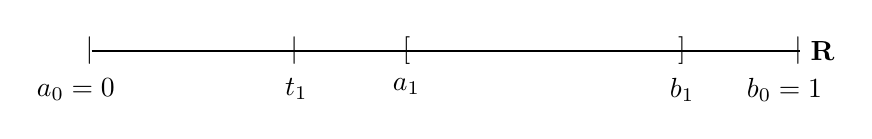
\begin{tikzpicture}
                    % Draw the number line with arrows on both sides
                    \draw[thick, ] (-3,0) -- (6,0) node[right] {$\mathbf{R}$};
                
                    % Mark points a and b
                    \filldraw (1,-0.23) node[below] {$a_1$};
                    \filldraw (4.5,-0.23) node[below] {$b_1$};

                    \filldraw (-3.2,-0.23) node[below] {$a_0 = 0$};
                    \filldraw (5.8,-0.23) node[below] {$b_0 = 1$};

                    \filldraw (-3.2,0) node[right] {$|$};
                    \filldraw (5.8,0) node[right] {$|$};

                    \filldraw (-0.6,0) node[right] {$|$};
                    \filldraw (-0.4,-0.23) node[below] {$t_1$};
                    
                
                    % Add parentheses around the interval (a, b)
                    \node at (1, 0) {$[$};
                    \node at (4.5, 0) {$]$};
                
                \end{tikzpicture}
            \end{center}
            Find $[a_1,b_1] \subseteq [0,1]$ with $t_1 \not\in [a_1,b_1]$. Find $[a_2,b_2] \subseteq [a_1,b_1]$ with $t_2 \not\in [a_2,b_2]$. Inductively, find $[a_n,b_n] \subseteq [a_{n-1},b_{n-1}]$ with $t_n \not\in [a_n,b_n]$. Thus $[a_n,b_n]$ is nested. Now let $\xi \in \bigcap_{n \geq 1}[a_n,b_n]$. Then $\xi \in [0,1]$. But $\xi \neq t_n$ for all $n$, which is a contradiction.
        \end{proof}

